Las Redes Tolerantes a Disrupciones (\textit{Delay Tolerant Networks} o DTN)
han llamado la atención de los investigadores debido a su potencial de permitir
comunicar a las personas sin la necesidad de una infraestructura de
comunicaciones centralizada. A continuación se presenta un estado del arte donde
se analizan las distintas publicaciones en DTN y se contrastan con la propuesta
de este trabajo.




\seccion{Redes tolerantes a disrupciones}

% Explicar una red ad-hoc

Con la intención de permitir la creación de redes de comunicación inalámbricas
sin necesidad de un punto de acceso es que se desarrollaron las redes ad-hoc
donde los nodos pueden actuar como enrutadores de los mensajes de comunicación.
Esta red debe ser capaz de formarse de manera rápida permitiendo la comunicación
sin necesidad de registrarse y manteniéndose independiente de cualquier
infraestructura \cite{ad-hoc}. Una DTN puede utilizar las redes ad-hoc como
forma de permitir la comunicación entre dispositivos y dado que es un estándar
se pueden conectar nodos heterogéneos mientras que el software lo permita. Otra
alternativa de comunicación es \textit{WiFi Direct}, un estándar parecido a las
redes ad-hoc pero para dispositivos Android, y conexión por medio de Bluetooth
que en los últimos estándares tiene rangos de comunicaciones comparables con
WiFi.

Las redes ad-hoc pueden ser clasificadas en Redes Ad-hoc Móviles (\textit{Mobile
Ad-hoc Networks} o MANETs), Redes Inalámbricas de Malla (\textit{Wireless Mesh
Networks} o WMNs), Redes Vehiculares Ad-hoc (\textit{Vehicular Ad-hoc Networks}
o VANETs), Redes Inalámbricas de Sensores (\textit{Wireless Sensor Networks} o
WSNs) y Redes Tolerantes a Disrupciones. Las MANETs \cite{MANETs} son redes que
permiten a los nodos auto-organizarse libre y dinámicamente en redes ad-hoc
temporales permitiendo a las personas comunicarse sin infraestructura previa a
la creación de la red.  Las WMNs \cite{WMNs} son parecidas a las redes MANETs
pero se enfocan en aplicaciones civiles por lo que pueden utilizar muchos de los
algoritmos desarrollados para MANETs. Las VANETs \cite{VANETs} son redes de
vehículos y tiene como objetivo la diseminación de mensajes de alertas en caso
de emergencias los cuales deben ser entregados a tiempo. Las redes de sensores
WSNs \cite{WSNs} son aquellas que se crean entre sensores de bajo costo
distribuidos en una área donde los mensajes deben realizar múltiples saltos
hasta llegar a una o más bases recolectoras teniendo en cuenta poca capacidad de
almacenamiento, poco ancho de banda y poca capacidad de cómputo. Finalmente, las
redes DTN se utilizan en situaciones donde hay conectividad esporádica.


% Explicacion de DTN

Las DTN fueron ideadas como una forma de comunicar los distintos dispositivos
utilizados en la exploración espacial ubicados fuera de la Tierra los cuales
deben poder enviar y recibir datos con los operadores, lo que dio origen a la
Internet Interplanetaria.  En esta hipotética red, protocolos típicos como
TCP/IP, utilizados para comunicar los computadores en la Internet terrestre no
pueden ser utilizados debido a que: existe una alta latencia de propagación,
baja tasa de transferencia, comunicación intermitente y los accesos al canal de
comunicación son manejados de manera centralizada.  Utilizar protocolos como TCP
requiere que tanto que el envía como el que recibe información negocien una
conexión que va a regular el flujo de datos, además si hay pérdida de datos
entonces se detiene el protocolo y se debe esperar hasta que se vuelva a
retransmitir. Utilizar UDP tampoco es factible dado que el manejo de la correcta
llegada de los datos se deja a la capa de la aplicación teniendo que reinventar
la retransmisión de TCP lo que es costoso. El protocolo propuesto para este tipo
de red se ubica entre la capa de aplicación y la de transporte dejando la
comunicación a bajo nivel a las interfaces correspondientes. Este protocolo
utiliza un concepto llamado \textit{store-and-forward} que consiste en almacenar
aquellos mensajes que no se pueden transmitir en un \textit{buffer} a la espera
de la próxima oportunidad de comunicación \cite{burleigh_delay-tolerant_2003}.


Otra aplicación que pueden tener las DTN es en comunicación terrestre donde no
se tiene acceso a una infraestructura de comunicaciones como Internet.  Algunos
casos de usos de este tipo de redes pueden ser: redes militares \textit{ad-hoc}
y redes de sensores, siendo todos estos casos de redes que tienen poca
conectividad y en algunos casos heterogéneas \cite{fall_delay-tolerant_2003}.
Estas restricciones han sido utilizadas para crear un protocolo llamado
\textit{Bundle}, que funciona como un \textit{overlay} entre la capa de
transporte y aplicación como se muestra en la \ref{gateway}.  Un servidor RPC
(\textit{Remote Procedure Call}) es ejecutado en cada uno de los nodos para
poder compartir información de la red como métricas o solicitar la compartición
de mensajes \cite{RFC5050}. Los intentos por parte de la IETF (\textit{Internet
Engineering Task Force}) de estandarizar este protocolo han desencadenado en la
creación de dos RFC (\textit{Request for Comments}) en el 2007: RFC 4838
\cite{RFC4838} y RFC 5050 \cite{RFC5050}, los cuales son una unión de ideas
obtenidas de trabajos previos realizados por el \textit{NASA Jet Propulsion
Laboratory} y otros investigadores del área.

\figuraFuente{Estructura un \textit{gateway} para DTN.}
{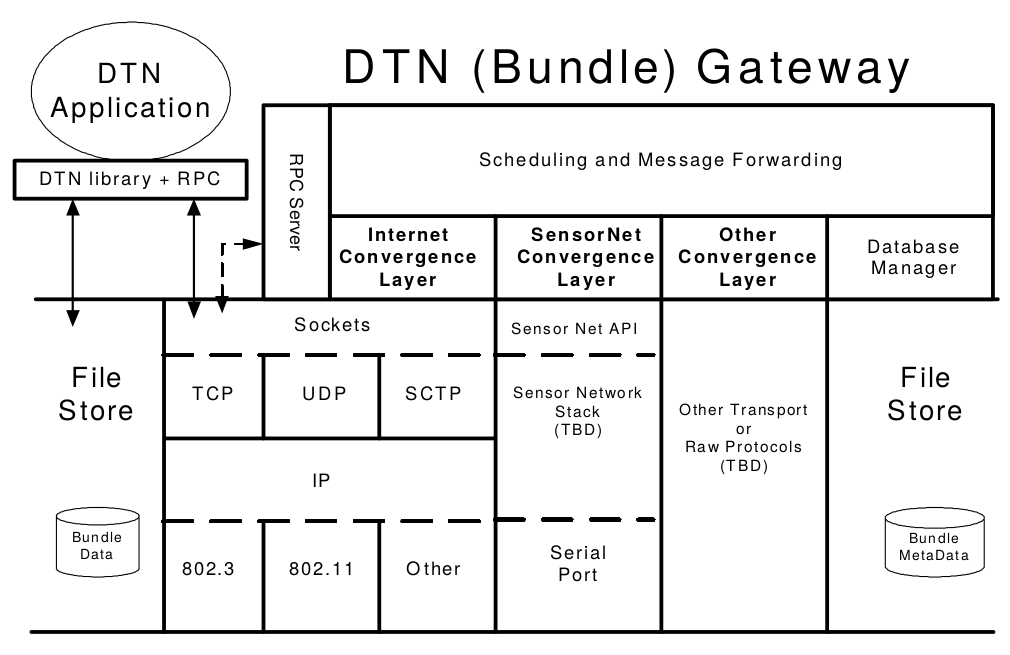
\includegraphics[scale=0.3]{imagenes/dtn/arquitectural_protcolo.png}}{gateway}
{Kevin R. Fall \cite{fall_delay-tolerant_2003}}


Una forma de modelar las DTN es mediante un grafo \cite{rapid} $G = (V, E)$
donde $V$ y $E$ representan un conjunto de nodos y aristas respectivamente.
Cada una de las aristas $e$ representa un encuentro o conexión entre nodos. Este
grafo va cambiando de acuerdo a las nuevas conexiones que se van creando
dependiendo de los rangos de comunicación que tengan los nodos. Este modelo
asume transferencias de datos cortas y discretas que caracteriza a varias DTNs
reales.



\seccion{Simuladores y evaluación de DTN}

Debido a que estas redes están pensadas para ser utilizadas con una gran
cantidad de nodos como en ciudades o pueblos medianos es que se hace difícil
poder probar estas redes en un ambiente real de manera replicable y que permita
las iteraciones necesarias para poder crear un buen protocolo. Por esta
razón se han desarrollado una serie de simuladores y métricas que permiten poner
a prueba los algoritmos de enrutamiento de una manera reproducible por los
investigadores en el área.

Uno de los simuladores más utilizados es \theone{} \cite{keranen_one_2009},
simulador hecho en java y uno de los más utilizado por las publicaciones en el
área. Permite probar nuevos protocolos y modelos de movilidad. Las métricas más
comunes de este simulador se encuentran en la clase \textit{MessageStatReport}
del simulador permitiendo el cálculo de tasa de entrega de mensajes a su
destino, copias redundantes hechas por el protocolo (\textit{overhead}) y
latencia.

\theone{} define un nodo DTN como un objeto dentro del sistema el cual tiene
asociado un protocolo, un modelo de movilidad y recursos para ejecutar el
protocolo. El protocolo es capaz de recopilar y calcular métricas para  decidir
si transmitir los mensajes o no a un nodo vecino.  El modelo de movilidad genera
rutas las cuales son seguidas por los nodos de acuerdo a una velocidad definida
en la configuración de la simulación.  Finalmente, los recursos que tiene
disponible un nodo incluyen el \textit{buffer} de almacenamiento de mensajes que
puede ser limitado o infinito, el rango de comunicación y la velocidad de
comunicación.

La tasa de entrega consiste en la cantidad de mensajes que han logrado llegar al
destino y se calcula de acuerdo a la ecuación (\ref{eq:delivery}) donde $d$ es la
cantidad de mensajes entregados (sin contar copias), $c$ es la cantidad de
mensajes creados en la red y $t$ es la tasa de entrega. Dado que en una red DTN
pueden existir copias de mensajes, se considera que un mensaje llega al destino
cuando la primera copia alcanza al nodo final.


\begin{equation}
    \label{eq:delivery}
    t = \frac{d}{c}
\end{equation}

Dado que una de las técnicas para transmitir mensajes en la red es la
realización de copias de los mensajes para aumentar la probabilidad de entrega
junto con reducir el riesgo de perder el mensaje debido a una caída de un nodo.
Estas copias de mensajes deben ser transmitidas desde un nodo a otro lo que
provoca dos problemas: aumento en el consumo de energía por la utilización de
comunicaciones inalámbricas y saturación de los \textit{buffers} de los nodos.
Es por esta razón que es importante medir cuantas copias se realizan en promedio
por los nodos de la red lo que se hace con la ecuación (\ref{eq:overhead}) donde
$r$ que es la cantidad de mensajes transmitidos, $d$ es la cantidad de mensajes
entregados al destino y $o$ es el \textit{overhead} de la simulación.


\begin{equation}
    \label{eq:overhead}
    o = \frac{r - d}{d}
\end{equation}


La latencia es el promedio de los tiempos que les tomó a los mensajes llegar a
su destino y debido a esta definición, solamente se consideran los mensajes que
han logrado encontrar el nodo receptor. La ecuación \eqref{eq:latencia} muestra
el cálculo de la latencia la cual es el promedio de los tiempos individuales de
cada mensaje donde $l$ es un vector que contiene el tiempo que le tomó al
mensaje $i$ llegar al destino y $n$ es la cantidad de mensajes que llegaron al
destino.


\begin{equation}
    \label{eq:latencia}
    T = \frac{1}{n}\sum_{i = 1}^n l_i
    %\tagaddtext{[s]}
\end{equation}


Para medir la energía se propone la ecuación (\ref{eq:energia})
\cite{martin-campillo_energy-efficient_2012} que relaciona el número de
contactos promedio por nodo $nc$ con la cantidad promedio de  mensajes
transmitidos por el nodo $x$ y el tiempo promedio de contacto por nodo $ct$.
Esta ecuación entrega un estimado de la energía utilizada por el nodo en Joules
por lo que se puede hacer una comparación entre los protocolos desde otro punto
de vista.


\begin{equation}
    \label{eq:energia}
    e(x, nc, ct) = 5.9(nc) + 0.007(x) + 0.05(ct)
    %\tagaddtext{[J]}
\end{equation}



En \cite{Sidera2016} se utiliza como base el \textit{Very Large DTN Simulator}
\cite{vl-dtn-simulator}, un simulador hecho en C que permite la ejecución de
simulaciones con una gran cantidad de nodos en un tiempo razonable, uno de los
principales problemas de \theone{}, llegando a poder simular sin problema 3000
nodos en un escenario. Sin embargo, es poco utilizado por la comunidad por lo
que tiene pocos protocolos y modelos de movilidad implementados.

Un simulador popularmente utilizado para todo tipo de redes es NS2 \cite{ns2}
que permite simular TCP, encaminamiento y \textit{multicast} sobre conexiones
por cable o inalámbricas (WiFi, Bluetooth y conexión por satélite). Este
simulador ha sido aplicado a redes DTN como sensores y redes móviles, pero en
este último en menor medida debido a la dificultad de crear modelos de movilidad
que simulen las desconexiones de los nodos en la red.






\seccion{Protocolos DTN}


Distintos protocolos han sido propuestos utilizando como base el estándar del
protocolo Bundle, es decir, actuando como un puente entre la capa de aplicación
y la capa de transporte y utilizan el concepto de \textit{store-and-forward}
para transmitir los mensajes.  Estos protocolos se diferencian principalmente
por la información utilizada en la decisión de encaminamiento como se muestra en
la \ref{protocolos-organizacion}.

Los protocolos deterministas conocen las futuras posiciones de los nodos que
componen la red y generalmente se aplican en situaciones como satélites donde
las órbitas pueden ser calculadas con precisión. En el caso de los protocolos
\textit{Space-time} estos modelan el problema de enrutamiento mediante grafos
espacio tiempo (\textit{space-time graphs}) donde se pueden calcular las rutas
más cortas para enviar el mensaje al destino tomando en cuenta la movilidad de
los nodos \cite{space-time}. Los protocolos \textit{Tree} crean un perfil de
movimiento de cada uno de los nodos de la red permitiendo el cálculo de
posiciones a futuro, utilizando esta información son capaces de construir un
árbol de caminos (\textit{Path Tree}) posibles desde la fuente hasta el destino
\cite{DBLP:conf/pervasive/HandoreanGR04}. Finalmente, los \textit{Modified
Shortest Path} son un conjunto de protocolos que disponen de oráculos que
proveen al protocolo de información como contactos, colas y tráfico de mensajes
de los dispositivos que los protocolos pueden utilizar para tomar decisiones de
encaminamiento utilizando algoritmos como Dijkstra
\cite{DBLP:conf/sigcomm/JainFP04}.


\figuraFuente{Protocolos según la información utilizada para la toma de decisiones.}{\begin{tikzpicture}
  [
    level distance = 1.5cm,
    every node/.style = { shape = rectangle, draw, fill = orange!40}, 
    level 1/.style = {sibling distance = 3cm},
    level 2/.style = {
      grow=down,
      text width = 10em,
      align = center,
      edge from parent path={(\tikzparentnode.south) |- (\tikzchildnode)},
    },
  ]

  \node {Protocolos DTN}
    [edge from parent fork down]
    child { node {Determinístico}
      child { node [xshift=-60pt] (primero) { \textit{Space-time} }}
      child { node [below of = primero] (segundo) { \textit{Tree} }}
      child { node [below of = segundo] (tercero) { \textit{Modified Short Path} }}
    }
    child { node {Estocástico}
      child { node [xshift=60pt] (primero2) { \textit{Epidemic} }}
      child { node [below of = primero2] (segundo2) { Predictivo }}
      child { node [below of = segundo2] (tercero2) { \textit{Model Based Routing} }}
      child { node [below of = tercero2] (cuarto2) { Control de movimiento }}
      child { node [below of = cuarto2] (quinto2) { \textit{Coding} }}
    }
  ;

\end{tikzpicture}
}{protocolos-organizacion}
{Elaboración propia basado en \cite{DBLP:phd/dnb/Mayer12a}}


Los protocolos estocásticos son una categoría donde los movimientos no pueden
ser calculados o solamente se pueden conocer con una precisión limitada.  Un
protocolo que no asume nada de la red y utiliza cero información son los
protocolos de inundación o \textit{Epidemic}. Otros protocolos pueden utilizar
la historia pasada para tratar de predecir la ubicación futura de los nodos
asumiendo que los movimientos son cíclicos tal es el caso de protocolos
\maxprop{} y \prophet.  Si se conoce más información sobre el movimiento de las
personas entonces es posible utilizar información como mapas de la ciudad para
mejorar los protocolos, esto se conoce como \textit{Model Based Routing}. Los
protocolos de control de movimiento pueden controlar hacia donde deben ir los
nodos de manera de poder entregar un conjunto de mensajes lo más rápido posible
al destino.  Finalmente, los protocolos \textit{Coding} asumen que pueden
mejorar los problemas de la red (pérdida de mensajes, falla de conexión, alta
latencia, etc) mediante distintas técnicas de programación como la replicación
de mensajes en distintos nodos para prevenir la pérdida de estos para lo cual
generalmente se utiliza una técnica de inundación.

En general el protocolo propuesto en este trabajo asume un entorno estocástico
en el cual es difícil de predecir las ubicaciones futuras de los nodos dentro
del área de movimiento y se va a ubicar en la capa \textit{Bundle} del modelo
presentado anteriormente.


Dentro de los protocolos DTN más utilizados en las publicaciones se encuentran:
\epidemic{}, \syw{}, \syf{}, \maxprop{} y \prophet{}, los cuales están pensados
para ser utilizados de manera genérica sin tomar en cuenta los diferentes
patrones de movilidad que puedan tener los nodos de la red.


\epidemic{} \cite{amin_vahdat_epidemic_2000} es un protocolo de comunicación que
consiste en transmitir los mensajes entre todos los nodos vecinos con la
esperanza de que luego de un tiempo los mensajes lleguen al destino. Cada vez
que un nodo se encuentra con otro intercambian una lista de mensajes
identificados por un ID único en el sistema, luego comparten entre ellos los
mensajes que faltan en el nodo vecino hasta que ambos tienen los mismos de
manera que con el solo movimiento de los nodos los mensajes van a comenzar a ser
transmitidos por la red hasta llegar al destino.  Esta inundación de mensajes
tiene como objetivo maximizar la tasa de entrega, minimizar la latencia y
minimizar el uso de CPU utilizado por el enrutamiento pero sin tomar en cuenta
los costos de transmisión de datos. Las simulaciones realizadas en este
protocolo muestran que tiene una tasa de entrega cercana al 100\% y dado que es
relativamente simple de implementar no consume una gran cantidad de recursos de
CPU. En simulaciones \cite{paper_evaluacion_nosotros} donde se limita el tamaño
del buffer y se calcula el consumo de energía de las transmisiones entonces es
uno de los protocolos que peor se desempeña gastando con un alto costo de
energía.

\syw{} \cite{spyropoulos_spray_2005} es un protocolo que trata de mejorar
\epidemic{} agregando un control a la inundación de mensajes. Consiste en dos
fases: una fase de \textit{spray} y una fase de \textit{wait}. Al momento de la
creación del mensaje en el nodo origen se le agrega un parámetro $L$ como
metadato según la configuración inicial del protocolo el cual va a indicar la
cantidad máxima de copias que va a tener el mensaje inicialmente. Cada vez que
un mensaje llega a un nodo receptor este parámetro $L$ es dividido por 2 hasta
llegar a 1 donde el protocolo comienza a ejecutar la fase de \textit{wait}
siendo ahora la única posibilidad de transmitir el mensaje es si se encuentra
con el destino final del mensaje, por eso esta fase recibe el nombre de
"espera". Esta forma de controlar el \overhead{} permite que \syw{} sea uno de
los protocolos con menor consumo de energía, pero también uno de los que tiene
peor tasa de entrega debido a que si se elije un $L$ pequeño en relación con la
cantidad de saltos hacia el destino entonces va ser necesario espera que los
nodos que tienen los mensajes se encuentren directamente con el destino que
puede llevar tiempo, haciendo además que sea uno de los protocolos con mayor
latencia en la entrega de mensajes.


\syf{} \cite{spyropoulos_spray_2007} es una mejora a \syw{} con el objetivo de
mejorar las tasas de entrega y altas latencias pero manteniendo el consumo de
energía bajo. Para lograr esto el protocolo realiza una fase de \textit{spray}
limitada por un parámetro $L$ que cuando el mensaje es pasado a otro nodo es
reducido en $L / 2$, es decir, ambos nodos quedan con $L / 2$ copias disponibles
para una siguiente fase de \textit{spray}. Cuando a un nodo no le quedan más
copias entonces pasa la la fase da \textit{focus} que a diferencia de la fase
\textit{wait}, si permite el paso de mensajes pero sin generar copia por lo que
el nodo que tenia el mensaje lo debe borrar de su buffer. Esta segunda fase se
caracteriza por utilizar tiempos transitivos para decidir si pasar el mensaje o
mantenerlo bajo el supuesto de: si un nodo $A$ ve al nodo $B$ frecuentemente y
el nodo $B$ ve al nodo $C$, entonces $A$ puede ser un buen candidato para enviar
un mensaje a $C$ por medio de $B$ aunque $A$ no vea frecuentemente al nodo
$C$. Estos tiempos transitivos se van distribuyendo en la red mediante
inundación. Finalmente, \syf{} obtiene mejores resultados en cuanto entrega de
mensajes que \syw{} y latencia al tomar en cuenta los tiempos transitivos pero
al costo de aumentar la transmisión de mensajes en la segunda fase por lo que
presenta un consumo de energía ligeramente más elevado que el protocolo
original.



\maxprop{} \cite{burgess_maxprop:_2006} es un protocolo basado en probabilidades
transitivas para la decisión de encaminamiento de los mensajes. Se tiene una
tabla de probabilidades inicializada en $\frac{1}{|s|-1}$  siendo $s$ el
conjunto de todos los nodos de la red.  Cada vez que el nodo se encuentra con
otros esta probabilidad es aumentada en 1 y luego se normaliza con todas las
probabilidades de la tabla usando un método conocido como \textit{incremental
averaging}. Cuando el nodo quiere evaluar que tan bueno es un vecino para
entregar el mensaje al destino genera un grafo utilizando la tabla de
probabilidades donde cada uno de los caminos entre los nodos tiene un costo dado
por el complemento de las probabilidades, por lo tanto el mejor camino es el
mínimo obtenido mediante algoritmos como Dijkstra. Este protocolo se diferencia
de los anteriores porque maneja además del paso de mensajes los \textit{buffers}
para evitar que se saturen y que los mensajes sean descartados, como en el caso
de \epidemic.  En el caso de un \textit{buffer} limitado este es uno de los
protocolos que mejor desempeño tiene pero al costo de tener un alto consumo de
energía, tanto en uso de CPU para el cálculo de caminos, como en costos de
transmisión.


\prophet{} \cite{lindgren_probabilistic_2003} \textit{Probabilistic Routing
Protocol} utiliza un enfoque parecido a \maxprop{} al utilizar las
probabilidades transitivas para evaluar si un nodo puede entregar un mensaje
mejor que otros o no. Esta probabilidad, llamada \textit{delivery
predictability}, es actualizada cada vez que se encuentran con un un nodo, pero
también si ha pasado un tiempo $k$, caso en el cual se reduce la probabilidad
utilizando una constante de envejecimiento $\upgamma$ que permite que las
probabilidades se actualicen en el tiempo. Para decidir si un mensaje es enviado
o no a otro, se compara la probabilidad de entrega del nodo local con la del
nodo del encuentro, si el otro nodo tiene mayor probabilidad de encontrarse con
el destino, entonces se pasa el mensaje, en caso contrario, el mensaje se
mantiene en el buffer local a la espera de encontrar un nodo que tenga mejor
probabilidad transitiva de entrega.  Este proceso implica una comparación y
cálculos matemáticos para las probabilidades por lo que es menos exigente
computacionalmente que \maxprop{}.  En cuanto al desempeño, este protocolo se
ubica a la par que \maxprop{} obteniendo tasas de entregas comparables con un
menor consumo de energía por transmisión de datos, pero de todas formas es
\maxprop{} el que obtiene las mejores entregas.


Una forma diferente de ver los protocolos DTN es pensar el problema de
enrutamiento como un problema de asignación de recursos como en el protocolo
\rapid{} \cite{rapid} donde se trata de responder a la pregunta de, dado un
ancho de banda limitado, ¿Cómo los mensajes deben ser replicados dado que se
optimice una de las siguientes métricas?: minimizar la latencia promedio y
minimizar los \textit{deadlines} (tiempo en que se espera la llegada de un
mensaje) perdidos, ambas definidas como una función de utilidad para
cada uno de los mensajes la cual es utilizada para decidir si replicar o no el
mensaje: el mensaje con mayor utilidad de la cola es replicado a los nodos
vecinos. Este trabajo además propone una manera de estimar la latencia promedio
con un algoritmo llamado \textit{Estimate\_Delay} que es utilizado para el
cálculo de la utilidad de una de las métricas.. Este protocolo fue probado en un
escenario vehicular que consistía en 40 buses, obteniéndose resultados que
muestran que Rapid puede entregar más rápido los mensajes que \maxprop{} y \syw,
y además con una mejor tasa de entrega utilizando la métrica para minimizar la
latencia promedio, sin embargo no hay pruebas respecto al
consumo energía del protocolo.


\textit{Encounter-Based Routing} (EBR) \cite{ebr} es un protocolo propuesto por
Nelson et al. que tiene como objetivo maximizar la tasa entrega mientras se
minimiza el \overhead{} siendo su algoritmo diseñado para reducir el consumo
energía utilizado por la CPU del dispositivo. Realizaron una clasificación de
los protocolos acuerdo a como tratan los mensajes ya sea simplemente
transmitiéndolos (\textit{forwarding-based}) o replicándolos
(\textit{replication-based}), siendo el primero aquellos protocolos que
mantienen solamente una copia del mensaje en la red.  Los protocolos que
replican sus mensajes a su vez pueden ser clasificados en dos subcategorías:
basados en cuotas (\textit{quota-based}) o basados en inundación
(\textit{flooding-based}), siendo un ejemplo del primero \syw. EBR es un
protocolo basado en inundación controlada mediante el conteno de la cantidad de
copias de mensajes que tiene disponible disponibles y tomando en cuenta la
cantidad de encuentros pasados de los nodos. El algoritmo funciona de la
siguiente manera: cada nodo mantiene dos variables dentro de su estado, el valor
del encuentro ($EV$) y la ventana actual de encuentros a ser considerada
($CWC$), donde $EV$ representa la tasa de encuentros pasados del nodo mientras
que $CWC$ es una ventana utilizada para solamente considerar una cierta cantidad
de encuentros recientes.  Cada vez que el nodo se encuentra con un vecino que
tiene un valor $EV$ desactualizado, $CWC$ es aumentado en uno.  Dado que $EV$
representa una predicción de la tasa de encuentros futuros del nodo basta con
comparar este valor local con el de un vecino para decidir si pasar un mensaje o
no, es decir, si el otro no tiene un valor $EV$ mayor, entonces se le pasan una
cantidad proporcional de copias del mensaje dado que tiene una mejor
conectividad en la red. Este protocolo se evalúa desde el punto de vista de la
tasa entrega y latencia contra otros protocolos de inundación como \maxprop,
\prophet, \epidemic, \syw{} y \syf, obteniéndose los siguientes resultados: EBR
tiene una mejor tasa de entrega de los demás protocolos probados, sin embargo,
presenta también la más alta latencia. Un punto a considerar es que no se
realizaron pruebas con respecto al consumo de energía que podría haber sido
medido indirectamente con el \overhead{} ni tampoco fue evaluado en un modelo de
movilidad orientado a desastres.


\tabla{Protocolos de acuerdo a la clasificación de EBR.}{
\pgfplotstabletypeset[
  columns/A/.style={column name=Clasificación, string type},
  columns/B/.style={column name=Protocolos, string type},
  every even row/.style={
  before row={\rowcolor[gray]{0.9}}},
  every head row/.style={ before row=\toprule,after row=\midrule},
  every last row/.style={ after row=\bottomrule},
  row sep=\\,
  col sep=&
]{
A & B \\
\textit{Quota-based}       & \syw, \syf, \prophet \\
\textit{Flood-based}       & \maxprop, \rapid, \epidemic \\
\textit{Forwarding-based}  & Protocolos tradicionales Ad-hoc y de Internet \\
}
}{tbl:clasificacion}
{Nelson et al. \cite{ebr}}












\newpage
\seccion{Modelos de movilidad}

% Hablar de los modelos de movilidad simples como random movement.


Una propiedad importante de las DTN es que son redes desconectadas que
aprovechan el movimiento de los nodos para poder entregar los mensajes. Si se
quiere desarrollar un buen protocolo para este tipo de redes es entonces
necesario entender como se mueven los nodos dentro de la red. Debido a que este
trabajo se enfoca en escenarios de desastres entonces es necesario poder modelar
como las personas se van a comportar en una situación de este estilo. A
continuación se presentan trabajos que han propuestos modelos de movilidad tanto
de personas como de vehículos dentro de ciudades afectadas por un desastre los
cuales pueden ser utilizados para el diseño y evaluación de  nuevos protocolos.

Nelson et al. \cite{Nelson2007} propuso un modelo de movilidad basado en
roles para modelar escenarios de desastres donde los nodos puede tener distintos
comportamientos. Se utiliza un modelo basado en fuerza donde los eventos tienen
una cierta "gravedad" que atraen o repelen a los nodos dependiendo de cual es
su rol en la simulación. Los nodos policías y rescatistas son atraídos hacia los
eventos, mientras que las personas comunes son repelidos. Existen horizontes de
suceso que marcan el límite de la influencia de los eventos en los nodos.
Mientras los nodos no son afectados por un evento, estos se mueven de manera
aleatoria por el escenario. Algunas métricas de evaluación utilizados para
probar el modelo de movilidad son: particiones en el tiempo, coeficiente de
\textit{clustering}, promedio de densidad en el tiempo, máxima densidad en el
tiempo y la varianza de la densidad de nodos en el tiempo. Estas métricas
permiten dar un perfil del modelo de movilidad utilizad y analizar que tan
exigentes son para los protocolos. Por ejemplo, un modelo de movilidad con un
alto coeficiente de clustering debería tener un protocolo probabilístico para
detectar si el destino se encuentra dentro del \textit{cluster} o no.

El coeficiente de \textit{clustering} es definido de acuerdo a la ecuación
(\ref{eq:clustering}) para un grafo no dirigido \cite{Watts1998}, donde $N_i$ es
la cantidad de vecinos del nodo $i$, $E$ es el conjunto de aristas que tienen
los nodos vecinos entre ellos y $k_i$ es el grado del nodo $i$. Este coeficiente
es una medida de que tan bien los vecinos del nodo se conocen entre ellos lo que
puede entregar un valor de que tan agrupada está la red. Un coeficiente de
\textit{clustering} de $1$ indica que la red está completamente conectado
mientras que un coeficiente de $0$ indica que esta se encuentra completamente
desconectada.

\begin{equation}
  C_i = \frac{2|\{e_{jk}\}|}{k_i(k_i - 1)} : v_j,v_k \in N_i, e_{jk} \in E
  \label{eq:clustering}
\end{equation}



Uno de los modelos de movilidad más utilizados en simulaciones es
\textit{Post-Disaster Mobility Model} o PDM \cite{uddin_post-disaster_2009} el
cual propone una serie de modelos de movilidad dentro de una ciudad tanto para
afectados, rescatistas, policías, ambulancias y centros de comando. El modelo
propuesto está definido en un periodo de $344000$ segundos o 4 días luego de que
un desastre golpeó una ciudad dividida vecindarios que contienen casas y cada
casa es el hogar de una o más personas. Las personas utilizan un modelo definido
como \textit{Human Movement} el cual al principio de la simulación elije una
casa que va a actuar como hogar. Luego de acuerdo a una probabilidad se decide
si se va a ir hacia un centro de evacuación o la persona se va a mantener en el
vecindario. En caso de ir hacia el centro de evacuación, entonces la persona se
va a mantener en la zona segura una cantidad de tiempo obtenida desde una
distribución una distribución de Pareto entre 24 a 48 horas.  Si la persona
decide quedarse en su vecindario, se va a mover en un radio $r$ al rededor de
su casa visitando a sus vecinos. Una vez se cumple el tiempo de permanencia en
el centro de evacuación las personas vuelven a su vecindario para realizar
rondas junto a aquellos que decidieron quedarse. Los rescatistas son personas
que se mueven a pie entre los centros de comando/evacuación base y un punto
aleatorio en los vecindarios de la ciudad creando un puente de conexión entre
las personas y las autoridades. Hay patrullas de policías que utilizan el
\textit{Patrol Movement} (\ref{fig:pdm-movimientos} (c)) el cual comienza
seleccionando un de las distintas estaciones de policías de la ciudad y luego se
mueve a un punto aleatorio del vecindario donde realiza una ronda para luego
volver al centro desde donde partió. Las ambulancias se mueven de una manera
similar, entre los hospitales y los vecindarios, pero dado que solamente
responden a llamadas de emergencia se quedan en el punto seleccionado y luego
vuelven (\ref{fig:pdm-movimientos} (b)). Hay otros vehículos que se describen en
el modelo de movilidad que ayudan a la logística luego de un desastre: vehículos
de suministros y de reparación de carreteras. Los vehículos de suministros se
mueven entre los centros de evacuación y el centro de comando para mover
alimentos y los vehículos de reparación se mueven entre los centros y cualquier
punto del mapa para reparar los posibles daños a la infraestructura.  Los nodos
de un vecindario se pueden ver en la \ref{fig:pdm-vecindario}, donde las
personas se encuentran moviéndose en su vecindario junto con un rescatista
(\textit{rescue worker}). Existen además vehículos con suministros que realizan
la función de conectividad entre los centros viajando entre ellos
(\ref{fig:pdm-movimientos} (a)). Este modelo de movilidad fue implementado para
el simulador \theone{} \cite{keranen_one_2009}.


\figuraFuente{Movimientos del modelo de movilidad PDM.}
{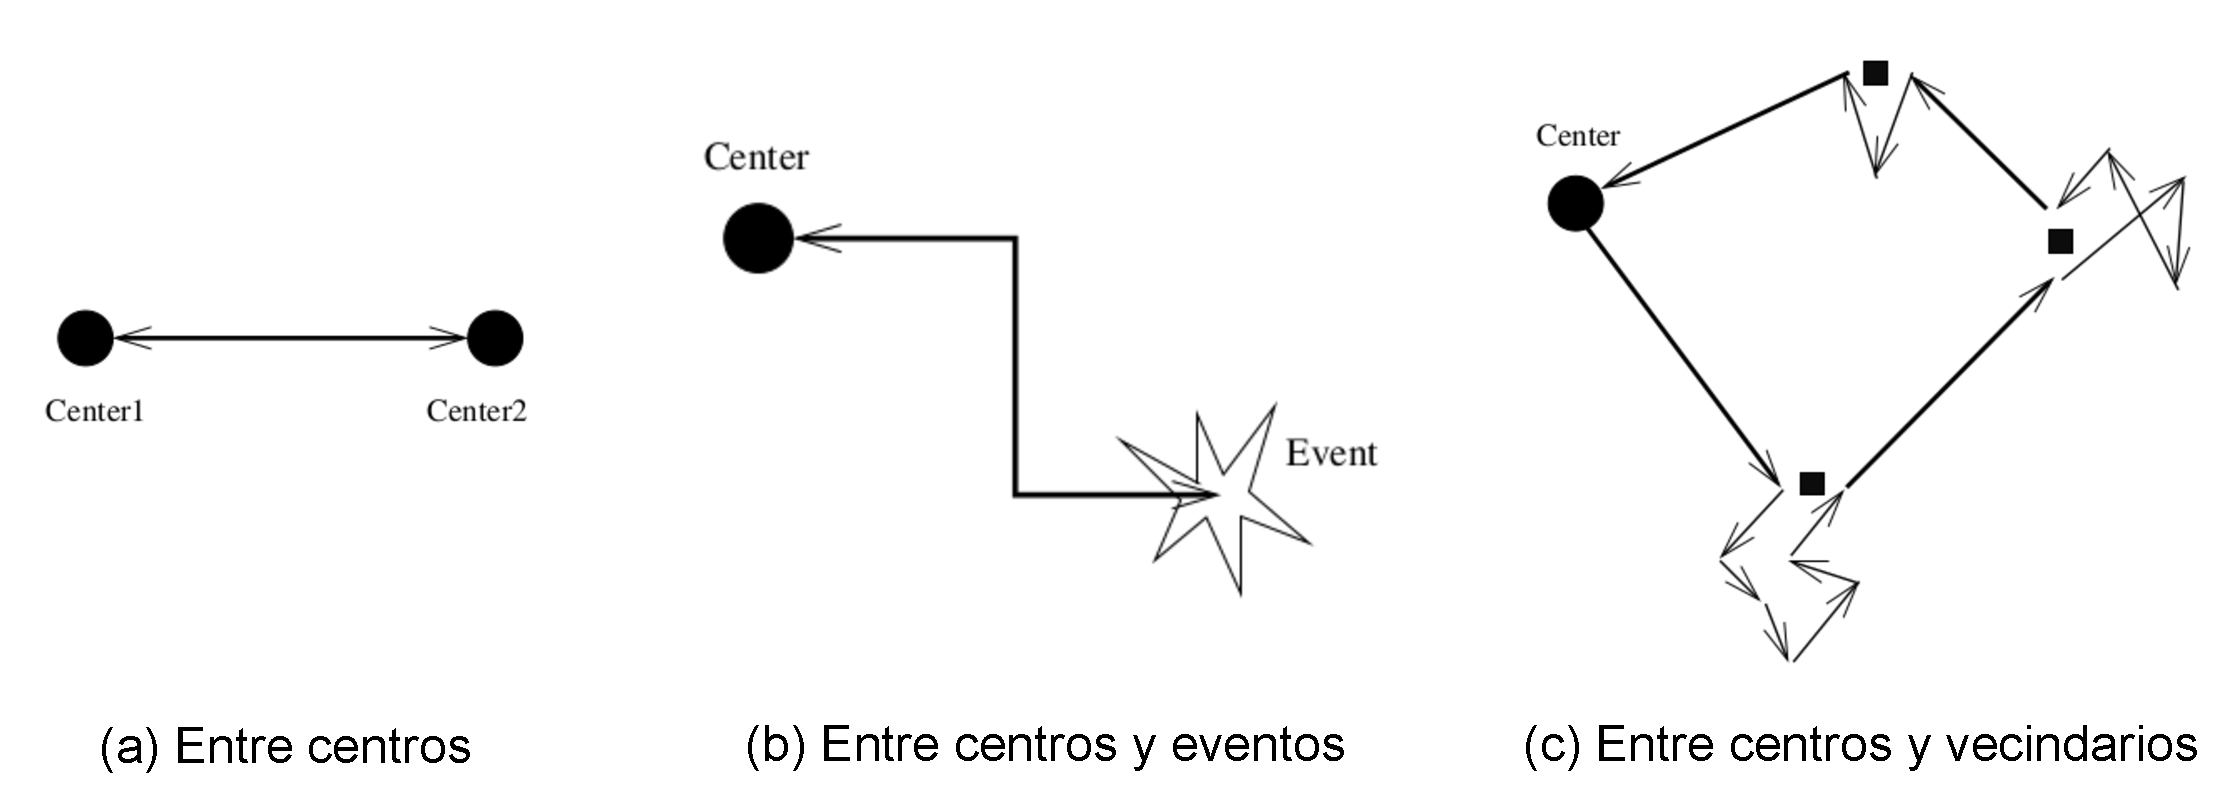
\includegraphics[scale=0.4]{imagenes/pdm/movimientos.eps}}{fig:pdm-movimientos}
{Uddin et al. \cite{uddin_post-disaster_2009}}



\newpage

\figura{Vecindario del modelo de movilidad PDM en el simulador \theone.}
{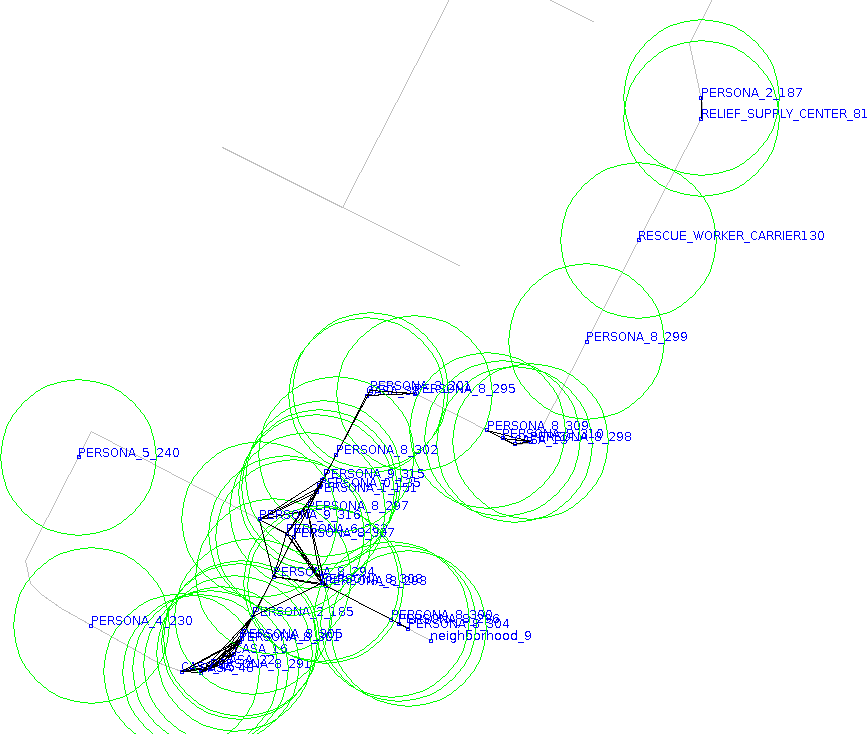
\includegraphics[scale=0.35]{imagenes/one/pdm_vecindario.png}}{fig:pdm-vecindario}





Similar a PDM es el \textit{Cluster Mobility Model} \cite{ozcan_post_2011} donde
existen grupos de nodos, que se pueden asemejar a vecindarios, y vehículos
que se mueven entre vecindarios creando la conexión entre cada conjunto, similar
a los vehículos de patrulla policial y ambulancias. Este modelo de movilidad
tiene como objetivo modelar un escenario de desastre donde cada uno de los
\textit{clusters} o grupos de personas se mueve de forma aleatoria en un punto
de interés como hospitales o refugios mientras que los \textit{carriers} o
vehículos conectan estos \textit{clusters} al transportar elementos de un lugar
a otro. A diferencia de PDM, este modelo de movilidad no está basado en mapas,
es decir las personas no se mueven por calles si no que en un espacio en blanco
sin ningún obstáculo como calles o edificios.



Otro modelo de movilidad orientado a escenarios de desastres es \textit{Disaster
Area} \cite{aschenbruck_modeling_2009} pero a diferencia del modelo anterior que
se enfoca en lo que ocurre en una ciudad completa luego de un desastre, este se
enfoca en un escenario más pequeño con una menor cantidad de nodos
participantes. Está basado en un desastre ocurrido en Colonia, Alemania donde
250 personas fueron heridas en un salón de eventos. Las áreas definidas en este
modelo son: lugar del incidente, área de tratamiento de heridos, zona de
transporte y zona de hospital. El área de incidente es el lugar donde ocurrió el
incidente desde el cual se van a evacuar las personas con ayuda de rescatistas.
Las personas afectadas son llevadas al área de tratamiento que consiste en dos
partes: área espera de tratamiento y zona de limpieza de causalidades. En la
primera área las personas esperan a ser transportadas al hospital medio de las
unidades de transporte (ambulancias y helicópteros) que esperan en una zona de
transporte. Para coordinar todas estas unidades se requiere de un centro de
control llamado comando de operaciones técnico ubicado en el área de tratamiento
de heridos. Debido a que la simulación puede tener obstáculos que impiden que
las unidades sigan caminos rectos es que se utilizan técnicas de planeación de
robots utilizando grafos de visibilidad para poder generar las rutas de las
unidades de transporte. Para la evaluación del modelo de movilidad se utilizaron
las métricas relacionadas con la cantidad de conexiones generadas por los nodos
dentro de la ciudad. A diferencia de PDM, DA no fue implementado como un modelo
de movilidad para \theone, si no que fue agregado a BonnMotion
\cite{DBLP:conf/simutools/AschenbruckEGS10}, un generador de trazas de
movimiento que pueden ser utilizadas en el simulador de DTN.


\textit{Working Day Mobility Model} \cite{ekman_working_2008} trata de modelar
una situación completamente distinta a los modelos anteriores ya que trata de
simular una ciudad en un día normal de trabajo. Este modelo se basa en varios
sub-modelos: \textit{Home Activity}, \textit{Office Activity}, \textit{Evenning
Activity} y \textit{Transport}. \textit{Home Activity} indica como los nodos se
mueven cuando se encuentran en sus casas en la tarde o en la noche donde se
mantienen quietos hasta que es hora de levantarse e ir trabajar. En
\textit{Office Activity} cada uno de los nodos tiene un escritorio y cada cierto
tiempo, definido por una distribución de Pareto, se mueven hacia un punto
aleatorio dentro de la oficina. Una vez las personas terminan de trabajar se
comienza con el modelo de \textit{Evenning Activity} que trata de simular
actividades como ir de compras, caminar por las calles o ir a un bar. Las
personas tienen un identificador que los hace pertenecientes a un grupo que
luego del trabajo se juntan en algún lugar de la ciudad a compartir. Una vez ha
pasado un tiempo definido en la configuración de la simulación, las personas
utilizan el modelo \textit{Transport} para volver a sus hogares a pasar la
noche. \textit{Transport} define tres sub-modelos de movimiento, \textit{Walking
submodel}, \textit{Car submodel} y \textit{Bus submodel}, donde cada persona
tiene una probabilidad utilizar cada uno de ellos para moverse por la ciudad.
Este modelo fue implementado en \theone{} en la ciudad de \textit{Helsinki},
Finlandia, y está pensado para simulaciones de 150 nodos. Algunas limitaciones
de este modelo como por ejemplo la posibilidad de modelar paredes u obstáculos
ni tampoco se agregaron normas del tránsito como límites de velocidad o
semáforos ya que esto implicaría la utilización de más recursos para simular la
ciudad.


Los modelos presentados anteriormente han sido creados desde un punto de vista
conceptual a partir de comportamientos anteriores de las personas frente a los
desastres, pero no han sido validados utilizando datos exactos sobre el
movimiento de las personas. En un trabajo reciente
\cite{10.1371/journal.pone.0147299} se analizaron publicaciones en
\textit{Twitter} geolocalizados de personas para obtener los patrones de
movimiento en desastres como tifones, terremotos, tormentas e incendios
forestales.  Dentro de los conjunto de datos para terremotos se incluyó uno del
terremoto de Iquique del 2014 con un total de 15297 \textit{tweets} de 1470
usuarios, una cantidad pequeña si se considera que el terremoto de Filipinas se
publicaron 114606 \textit{tweets} de 7942 usuarios por lo que no es muy
representativo del movimiento de las personas cuando existen rutas definidas de
evacuación como en Chile, pero si se puede descubrir un modelo general del
movimiento de las personas cuando no hay entrenamiento de la población sobre los
lugares seguros de la ciudad. Luego de analizar los \textit{tweets} y
movimientos de las personas se descubrió que estos siguen una ley de potencia,
es decir, la mayoría de las personas se comportan de una manera similar mientras
unas pocas se diferencian del resto, además existe una correlación de los
movimientos de las personas en un estado tranquilo comparado con un estado
alterado, pero no es así cuando ocurre un gran desastre donde el movimiento de
las personas se vuelve errático. Este estudio confirma los modelos anteriores
donde las personas se mueven de manera aleatoria en su vecindario por la ciudad
en caso de desastre.


Dado que los movimientos de los rescatistas depende en su mayor parte del tipo
de desastre ante el cual están acudiendo es que se requiere un modelo de
movilidad que esté basado en una situación en particular. En
\cite{krug_movement_2014} se hace un estudio de dos escenarios de desastres
reales para los cuales se derivó: un incendio en un edificio y una búsqueda de
persona desaparecida. El incendió contó con la participación de 260 bomberos y
duró 38 horas divididas donde al principio los bomberos entran al edificio
tratando de apagar zonas focalizadas. Existe un centro de comando que
coordina el trabajo de los bomberos y participación de policía y ambulancias. El
escenario de búsqueda de persona consiste en una gran área donde seis equipos
compuestos por personas y perros rescatistas se mueven llegando a un total de
aproximadamente 100 nodos. 



Gondaliya et al. \cite{Gondaliya2015} realizó evaluaciones de protocolos DTN en
escenarios de desastres, específicamente utilizando el modelo de movilidad PDM
en el simulador \textit{The ONE}, con el objetivo de ver el comportamiento de los
protocolos en estas situaciones en una ciudad. Se evaluaron tasa de entrega,
latencia, tasa de \textit{overhead} y saltos promedio de los mensajes. Se
evaluaron \epidemic, \prophet, \ebr, \syf{} y \syw. Las pruebas consistieron en
evaluar como las diferencias en el tamaño del \textit{buffer} afectan a los
protocolos como también distintos tamaños de mensajes y cantidad de mensajes en
la red. La conclusión a la que se llegó en este trabajo fue que un tamaño óptimo
del \textit{buffer} es de $35M$ para los protocolos \epidemic{} y \prophet,
mientras que estos mismos son los que tienen mayor tasa de entrega para el caso
de mensajes de tamaño $256KB$. \syw{} y \ebr{} tienen una tasa de entrega igual
sin importar el tamaño de los mensajes.


En un \textit{survey} realizado recientemente por Rosas et al. \cite{survey} se
hace un estudio del estado del arte de las simulaciones de DTN desde protocolos
hasta modelos de movilidad. Dentro de los modelos presentados están los que ya
fueron presentado pero se incluyen cinco más los cuales fueron clasificados de
acuerdo a si eran basados en mapas, basados en eventos, si contenían obstáculos,
si tenían movimientos en grupo, si se basaba en la definición de áreas y si
tiene movimientos heterogéneos, es decir, distintos tipos de nodos con
distintos tipos de movimiento. En la \ref{tbl:modelos_movilidad} se hace hace
reproduce la tabla del \textit{survey} para los modelos de movilidad ya
presentados.


\tabla{Características de los modelos de movilidad.}{

\pgfplotstabletypeset[
  columns/A/.style={column name=Modelo, string type},
  columns/B/.style={column name=Mapas, string type},
  columns/C/.style={column name=Eventos, string type},
  columns/D/.style={column name=Obstáculos, string type},
  columns/E/.style={column name=Grupos, string type},
  columns/F/.style={column name=Áreas, string type},
  columns/G/.style={column name=Movimientos, string type},
  every even row/.style={
  before row={\rowcolor[gray]{0.9}}},
  every head row/.style={ before row=\toprule,after row=\midrule},
  every last row/.style={ after row=\bottomrule},
  row sep=\\,
  col sep=&
]{
  A & B & C & D & E & F & G\\
  Disaster Area          &       &         & X           &        & X     & X \\
  PDM                    & X     &         &             &        &       & X \\
  \textit{Cluster}       &       &         &             & X      &       & X \\
  \textit{Working Day}   & X     &         &             & X      & X     & X \\
}
}{tbl:modelos_movilidad}
{Rosas et al. \cite{survey}}








\seccion{Protocolos orientados a desastres}

Los protocolos presentados anteriormente \protocolos, fueron diseñados
pensando en la aplicación a DTN genéricas, por lo que no toman en consideración
problemas que puedan existir en escenarios de desastres como poca disponibilidad
de la energía de los dispositivos y además, como se mostró anteriormente, si es
que un protocolo tiene más información sobre el escenario en el cual se está
ejecutando, entonces es posible mejorar el desempeño de este.


\textit{Time to Return} (TTR) \cite{Mart2009} es un protocolo que fue construido
con el objetivo de solucionar el problema de triaje \footnote{El triaje, del
francés triage o clasificación, es el problema de clasificar pacientes en
emergencias o desastres.} que comúnmente es solucionado mediante códigos de
colores de acuerdo a la gravedad de las heridas. El protocolo funciona de la
siguiente manera: cada vez que una persona sale del centro de comando se le
asigna un tiempo en el cual debe volver. A medida que avanza por la zona de
desastre y va recolectando información, cada vez que se encuentra con otro
dispositivo se comparan los tiempos de retorno, si el tiempo del otro es menor
(debe volver antes) entonces los mensajes son pasados a él para que lleguen lo
más pronto posible al centro de comando, en caso contrario se reciben los
mensajes del otro nodo. Se hizo una comparación
\cite{martin-campillo_evaluating_2013} entre \maxprop{}, \epidemic{}, \prophet{}
y \ttr{} donde uno se mostró que protocolos que saturan el \textit{buffer} como
\epidemic{} o \prophet{} bajan su tasa de entrega mientras que aquellos que
tratan de controlar el \overhead{} como TTR y \maxprop{} tienen una mejor tasa
de entrega a medida que aumenta la densidad de nodos. A pesar que hay un estudio
del \overhead{} de mensajes en las simulaciones, no existe una comparación del
consumo de energía realizado por los nodos.


En un desastre natural es común que se quiera enviar un mensaje a todos los
participantes de la red, utilizar \textit{multicast} o inundación es una solución
sencilla de realizar pero rápidamente llena los \textit{buffers} de los nodos y
no se puede garantizar que el mensaje llegue a todos. El protocolo RMDA
(\textit{Reliable Multicast over Delay Tolerant Mobile Ad hoc Networks})
\cite{DBLP:conf/msn/BegerowKSS14} permite hacer \textit{multicast} de los
mensajes de una manera eficiente y confiable pero además permitiendo el envío a
nodos individuales. Para funcionar asume que hay pequeños grupos de personas que
forman una MANET y estos grupos se comunican entre ellos mediante DTN, los nodos
entran a la red al momento del desastre y permanece en el hasta el final y si se
compara el tráfico de \textit{multicast} con el de \textit{unicast}, este último
es mayor comparado con el otro. El manejo del buffer lo realiza dando más
prioridad a los mensajes \textit{multicast}, pero cada vez que llega un nuevo
mensaje que requiera ser enviado a todos los nodos de la red, se elimina el
mensaje \textit{multicast} más viejo del \textit{buffer}. Para que el protocolo
sea confiable se utilizan ACKs de respuesta para confirmar la recepción de los
mensajes y poder hacer espacio en el \textit{buffer}.  El protocolo fue simulado
en \theone{} variando densidad de nodos y tamaño del buffer comparándolo con
\epidemic{} donde obtiene una mejor tasa de entrega de mensajes
\textit{multicast}. Begerow et al. propuso una mejora para RMDA \cite{Begerow2015}
añadiendo una tasa de entrega variable y un mecanismo para entregar mensajes de
manera selectiva permitiendo a los mensajes seleccionar un nivel de tasa de
entrega. A diferencia del protocolo anterior, existen tres niveles de
\textit{buffers} distintos cada uno asignado un rango de tasa de entrega de
acuerdo a la configuración del mensaje. Esta y la anterior implementación se
compararon mostrando una mejora en la tasa de entrega de mensajes
\textit{multicast} pero aún siguen sin existir comparaciones con otros
protocolos más utilizados ni consumo de energía.


Con el objetivo de enviar mensajes desde las personas hacia los oficiales
encargados de solucionar los problemas causados por el desastre es que Kawamoto
et al. \cite{Kawamoto2015} propone reducir la redundancia de mensajes
(\overhead). En este trabajo se hizo primero una experimentación para tratar de
entender qué dificultades tenían los protocolos en un escenario de desastre,
especialmente \epidemic. Se descubrió que mensajes en ciertas áreas de la
simulación no eran entregados con una alta probabilidad por lo tanto una mejora
podría ser evitar la transmisión de mensajes en las áreas que se sabe que se va
a obtener poca probabilidad de entrega. Finalmente, el protocolo propuesto
consiste en el cálculo de distancias hacia el destino siguiendo una ruta ideal
pero si la distancia es más grande que un umbral entonces el mensaje es
descartado. Se hicieron experimentos midiendo el \overhead{} y la tasa de
entrega de mensajes obteniendo resultados que son mejores que el protocolo
original pero en algunos casos \epidemic{} sigue siendo el mejor protocolo en
esta situación.  Éste es un ejemplo de un protocolo que requiere saber mucha
información sobre el escenario en que se está moviendo requiriendo el uso de
dispositivos GPS lo cual es poco realista si es que se tiene como objetivo la
reducción del consumo de energía. 

Un país que sufre desastres naturales parecidos Chile es Japón, país que por el
terremoto y tsunami de 2011 fue dañado en su infraestructura de comunicaciones
las cuales quedaron destruidas o dañadas tomando alrededor de un mes para que
fueran reparadas. Según el trabajo de Yamashia et al. \cite{Yamashita2015} las
mayores dificultades de las redes DTN son mejorar la tasa entrega y el consumo
energía por lo que Yamashita et al. propone un nuevo protocolo capaz de
enfrentar estas dificultades.  El objetivo principal de este protocolo es la
entrega de mensajes desde las personas hacia un refugio con el objetivo de
realizar confirmaciones de que las personas se encuentran bien evitando la
cantidad de inundaciones de mensajes, el consumo energía y el almacenamiento de
mensajes de los dispositivos. El protocolo funciona de la siguiente manera: los
rescatistas se clasifican como terminales de carga que llevan los mensajes desde
las personas hacia los refugios, por lo tanto Yamashia et al. se centran en la
reducción de energía de los terminales de los voluntarios minimizando la
cantidad de mensajes generados en la red y la cantidad de saltos que deben
realizar estos mensajes.  Existen tres tipos de mensajes: mensaje de búsqueda,
mensajes de respuesta y \textit{ACK}. El dispositivo del rescatistas envía un
mensaje de búsqueda cada $T$ segundos y cada vez que una persona recibe este
mensaje responde con uno de respuesta por el tiempo actual y sus coordenadas
GPS, por lo tanto no existe paso de mensajes entre una persona y otra, solamente
entre el rescatistas y personas o entre rescatistas y centros de comando. Este
protocolo es específico el escenario ya que tiene comunicación de una sola vía,
a que los mensajes se encuentran predefinidos dentro de la aplicación y a que se
utiliza el GPS que no es considerado como gasto de energía del protocolo por lo
que realmente puede que este protocolo no reduzca el consumo de los
dispositivos.

Una propuesta de arquitectura de red es propuesta por Gupta et al. \cite{Gupta2015},
donde se definen cuatro categorías para una red heterogénea de dispositivos los
cuales son: \textit{tier-1} (Voluntarios), \textit{tier-2} (\textit{Throw
boxes}), \textit{tier-3} (Vehículos) y \textit{tier-4} (Centro de comando).
Esta clasificación permite modelar más fácilmente los distintos dispositivos que
van a estar interactuando en el escenario desastre.  El protocolo propuesto
consiste en utilizar la dirección del movimiento del nodo, llamada factor
direccional calculada mediante una fórmula de distancia desde la posición actual
hacia el destino, posición conocida con anterioridad dado que los nodos que se
mueven dentro del escenario son rescatistas. Esta distancia es calculada entre
intervalos de tiempo por lo que es posible determinar si es que el nodo se está
moviendo hacia el destino o desde el destino. Una fórmula utilizada para
calcular la medida basada en esta distancia para decidir si el mensaje debe ser
mantenido por el nodo o entregado a un nodo vecino. Los autores realizaron
pruebas que fueron realizadas respecto a la tasa entrega, latencia, \overhead{} y
mensajes descartados. Estos resultados muestran que el nuevo protocolo tiene una
tasa entrega similar a la de \maxprop, \rapid{} y \ebr, una latencia mucho menor,
\overhead{} promedio y pocos mensajes descartados en comparación con los
protocolos probados. Otras pruebas consistieron en analizar como el protocolo se
comporta de distintas densidades de nodos mostrando que el protocolo tiene una
escalabilidad parecida al resto.  Este protocolo muestra que utilizando más
información del escenario, en este caso la dirección del movimiento y las
posiciones de los nodos, es posible mejorar las tasas de entrega y consumo de
energía respecto a los protocolos más generales pero no tomar en cuenta que el
uso del GPS es un dispositivo caro de mantener funcionando, especialmente en un
escenario desastre y en un dispositivo móvil, por lo que la práctica no es
viable utilizar este protocolo.


Con el fin de compartir información sobre la necesidad de comunicación de las
personas con las autoridades de que se propone por parte de Basu et al.
\cite{Basu2016} el uso de las características de la movilidad de las personas:
localidad espacial y regularidad espacial. La localidad espacial hace referencia
a que los voluntarios encargados de realizar operaciones en el área desastre se
suelen mover dentro de una  área local, mientras que la regularidad espacial
visitan periódicamente algunas otras áreas. Similar al modelo de movilidad PDM,
el área desastre es organizada en vecindarios los cuales son comunicados por los
rescatistas quienes a medida que avanzan por la ciudad van recolectando las
necesidades de las personas. Una vez el rescatista ha terminado su ronda, vuelve al
vecindario que es considerado como su hogar (debido a la regularidad espacial)
donde comparte esta información con los demás nodos rescatistas de esa
región (vecindario) y ahora cuando alguno de sus nodos se encuentre con la
estación de control (autoridades) para entregar información actualizada sobre
las necesidades de las distintas zonas de la ciudad. Las pruebas se basaron en
un desastre natural ocurrido en India sin realizar mediciones del consumo de
energía del protocolo.

Un conocido problema de los protocolos DTN es la pérdida de mensajes guardados
en los buffers debido a la limitada capacidad de almacenamiento que tienen los
dispositivos utilizados en este tipo de redes lo que puede provocar la pérdida
de mensajes importantes dentro del sistema. Para solucionar esto Bhattacharjee
et al.  \cite{Bhattacharjee2016}  propone \textit{PenPRoPHET}, un protocolo que
separa los mensajes entre los que tienen una alta prioridad de los que tienen
una baja mediante el procesamiento de lenguaje natural aplicado a cada uno de
los mensajes que llegan al dispositivo. Se utilizó un modelo de clasificación
entrenado mediante mensajes de texto intercambiados por los voluntarios en
situaciones de emergencia previa dándole cada mensaje una categoría de entre
cinco. Para la transmisión de mensajes se utilizó en el protocolo \prophet{} con
una modificación para incluir en su toma decisión la prioridad de los mensajes
mediante una métrica llamada Forwarding Priority que mezcla probabilidad de
entrega de los mensajes calculada por el protocolo con la prioridad del mensaje
estimada según el clasificador. Realizaron simulaciones utilizando el modelo
de movilidad PDM para comprar el nuevo protocolo creado, \textit{PenPRoPHET} con
\prophet{} sin modificar y otros protocolos del estado del arte como \maxprop,
\syw{} y \epidemic.  Los resultados mostraron que el nuevo protocolo es capaz de
entregar con mayor probabilidad aquellos mensajes con una prioridad alta
mientras que los demás protocolos tradicionales no muestran una preferencia por
ninguno de las cinco categorías de prioridad.  El protocolo sufre un problema
debido a que la priorización de los mensajes solamente se hace con datos de
prueba de voluntarios que están participando en la simulación no necesariamente
con personas comunes quienes también pueden ser beneficiadas de participar en la
red y de enviar y recibir mensajes situación que no es tomada en cuenta en este
trabajo. Además, no se hizo un estudio del posible consumo de energía del
clasificador el cual puede tener un gran impacto en la duración de la red.


\seccion{Protocolos orientados al contexto}

Los protocolos sensibles al contexto (context-aware) son aquellos que utilizan
su entorno para adaptarse a la situación actual del nodo. A diferencia de los
protocolos tradicionales que suelen utilizar probabilidades de encuentro para
decidir si entregar un mensaje de comunicación o no, los protocolos sensibles
al contexto utilizan más información, como densidad de los nodos, capacidad de
los \textit{buffers} o velocidad de movimiento.

Lakkakorpi et al. \cite{DBLP:conf/mswim/LakkakorpiPO10} propuso una mejora a
las redes MANET utilizando DTN cuando el contexto indica una baja densidad de
nodos. La densidad lo nodos se calcula mediante el uso del protocolo ad hoc
que permite identificar la cantidad de nodos vecinos que tiene el nuevo
actual, el cual si es menor que un umbral entonces el protocolo decide enviar
el mensaje mediante DTN. Este protocolo presentado utiliza el contexto o
situación actual para tomar una decisión dentro de la red, en este caso
utiliza la densidad de los nodos.

Boldrini et al. \cite{DBLP:journals/jnca/BoldriniCDP10} propone un protocolo
que utiliza los contextos para predecir los movimientos futuros de los usuarios
ayudándose además con información social. El contexto del usuario consiste en
dos conjuntos separados de información: el primero tiene que ver con información
personal del usuario (nombre, dirección, lugares más visitados, etc), mientras
que el segundo mantiene información social en términos de un grafo de conexiones
entre usuarios.  Además de estos contextos, existe el contexto del dispositivo
que está principalmente relacionado a las características físicas y limitaciones
que tiene en términos de capacidad, batería y tecnologías disponibles.
Utilizando esta información disponible el protocolo puede entregar los contextos
a lo largo de la red los cuales pueden ser utilizados para la toma de decisiones
de enrutamiento que consisten en una función de utilidad respecto al mensaje a
ser enviado en el contexto existente.


Cabacas et al. \cite{DBLP:journals/ijflis/CabacasR14} presentaron CMP
(\textit{Context Information-based Routing Scheme with Energy-based Message
Prioritization}) que utiliza los contextos de los nodos para decidir si pasar el
mensaje a un nodo vecino o no. Los contextos utilizados son: historial de
contactos (lugar y tiempo) y velocidad, los que permiten calcular hacia el lugar
donde se dirigen los nodos con el objetivo de ver que tan buenos son para la
transmisión del mensaje. Este es un protocolo determinista puesto que los nodos
conocen sus posiciones y velocidades por lo que es posible calcular las
posiciones futuras. El mensaje luego es pasado a un nodo que tenga como
trayectoria el destino del mensaje dentro del escenario. Este protocolo tiene la
desventaja de funcionar mediante el conocimiento de la velocidad y destino del
nodo, cosa que en un dispositivo móvil como un celular se podría averiguar
solamente con el uso de GPS, cuyo consumo de energía restringe su uso en
escenarios de desastres.



CAR es un protocolo propuesto por Musolesi y
Mascolo\cite{DBLP:journals/tmc/MusolesiM09} para redes ad hoc que utiliza
contextos definidos como un conjunto de atributo que describe los aspectos del
sistema para tomar la decisión de encaminamiento. Un contexto es definido en
forma de n-tupla $(X_1, X_2, ..., X_i)$ donde cada elemento es un atributo. Los
nodos calculan la utilidad de transmitir el mensaje a partir de los atributos
que componen el contexto actual tanto del nodo local como de los nodos vecinos.
Utilizando estos datos el protocolo es capaz de adaptarse a distintas
condiciones de la red como la cantidad de saltos realizados por los mensajes
aplicando cada uno de estos contextos a unas funciones de utilidad. Una vez
evaluado el contexto con las funciones de utilidad, se busca maximizar la
utilidad entregada de acuerdo a un peso que le entrega mayor importancia a
ciertas utilidades que otras. Finalmente el mensaje es entregado a aquel nodo
que pueda maximizar más la utilidad de entregar el mensaje de acuerdo al
contexto actual.  Oliveira et al. \cite{DBLP:journals/ijwin/OliveiraSPNMMA16}
proponen CARTOON (\textit{Context-aware Routing Protocol for OppOrtunistic
Networks}) donde se utilizan los contextos de la red para adaptar los parámetros
del protocolo. La idea del protocolo es cambiar entre dos modos: un modo
epidémico si es que hay una densidad baja de nodos y un modo probabilístico en
caso de tener una densidad alta. Este protocolo se comporta de mejor manera que
los protocolos definidos en el estado del arte que tienen una configuración
estática para todos los nodos de la red.



\seccion{Redes y protocolos híbridos}

Debido a la diversidad de dispositivos que participan en redes DTN
(heterogéneas) es que se han propuestos mezclas tanto de arquitecturas como de
protocolos, con el fin de mejorar las tasas de entrega o el consumo de energía.
Dentro de los tipos de arquitecturas que se han propuesto hay unas que mezclan
redes DTNs con MANETs, ad hoc e Internet, mientras que por el lado de los
protocolos se han mezclado protocolos que utilizan distintas estrategias para la
entrega de mensajes de acuerdo a la composición de la red.


\subseccion{Redes híbridas}

Una alternativa a los protocolos DTN en escenarios de desastre son las MANET
formadas a partir de redes Ad Hoc las cuales permiten una mejor tasa de entrega
al asumir que existe una conexión constante a lo largo de la red, situación que
la mayoría de los casos no puede cumplirse. Mezclar ambos tipos de arquitecturas
de redes puede permitir una alta tasa de entrega en vecindarios pero al mismo
tiempo soportar las disrupciones propias de un escenario desastre. Para lograr
esto se propone \cite{Raffelsberger2013} agregar el paradigma de
store-and-forward a los protocolos Ad Hoc que va a ser utilizado en el caso que
no exista una ruta hacia el destino, momento en el cual el mensaje es guardado
en un buffer hasta que nuevamente la ruta vuelve a estar disponible y los
mensajes son enviados de acuerdo a la regla FIFO (first in, first out). para las
pruebas se modificaron los protocolos de redes MANET, BATMAN y OLSR, pero estas
fueron realizadas de manera simple sin mostrar ninguna comparación con
protocolos DTN del estado del arte por lo tanto no es posible decir si realmente
existe una mejora con esta solución.

Con el objetivo de mejorar la latencia se han realizado experimentos para
mezclar DTN con las infraestructuras de comunicaciones como Internet, donde es
posible aprovechar esta vía de comunicación para ir de un lugar a otro de la red
que estén separados por muchos saltos entre nodos \cite{mayer_routing_2014}. En
un escenario de desastre pueden existir nodos con acceso Internet los cuales
pueden ser utilizados como punto de acceso por lo que el protocolo puede ahora
tomar la decisión de ver si utilizar Internet o utilizar los saltos entre nodos
para entregar el mensaje (la DTN). Cada uno de los nodos que tiene acceso
Internet es parte de una DHT (\textit{Distributed Hash Table}) donde lo nodos
vecinos utilizada para guardar información sobre que nodos son adyacentes con
quien. Resultados de simulaciones demostraron que es posible mejorar el
desempeño de redes mediante el uso Internet y especialmente la latencia, pero es
poco realista asumir que Internet va estar disponible en un escenario desastre y
además no es una solución completamente distribuida ya que los nodos deberían
conocerse de antemano para por ser parte de la red DHT o primero conectarse a un
servidor que les permita encontrarse.




\subseccion{Protocolos DTN híbridos}

Los protocolos DTN híbridos son aquellos que mezclan dos o más protocolos
previamente definidos en uno solo bajo una regla que suele ser una
heurística. A continuación se presentan algunos protocolos que utilizan este
concepto para mejorar algunos parámetros de los protocolos. Hay que aclarar que
otros autores se refieren a las redes híbridas como protocolos híbridos mientras
que en este trabajo se habla a nivel de las reglas de enrutamiento y no de la
arquitectura de la red.


Los mismos investigadores que propusieron el protocolo TTR se dieron cuenta que
existía la oportunidad de integrarlo con el uso de las probabilidades de un
protocolo como \maxprop{} con el objetivo de mejorar la tasa entrega del
protocolo original \cite{martin-campillo_energy-efficient_2012}. Uno de los
problemas que tiene TTR es que es si se encuentra con un nodo que tiene un
tiempo de retorno menor entonces el mensaje será transferido teniendo en cuenta
la posibilidad de encontrarse con un nodo a futuro que puede tener una mejor
probabilidad de entrega. \maxprop{} es utilizado en una primera etapa dentro del
protocolo para realizar copias de los mensaje de acuerdo a las probabilidades
transitivas mientras que el siguiente salto del mensaje se utiliza TTR como está
definido originalmente. Debido a estos dos protocolos se ejecutan en uno solo,
es necesario mantener el estado separado dependiendo de cual es el que está
siendo ejecutado en el momento. Los resultados experimentales muestran una
mejora significativa en la tasa entrega pero manteniendo un costo (\overhead)
similar al protocolo original, pero a pesar de esto, este protocolo sigue
teniendo una aplicación muy limitada dado que depende mucho del movimiento que
tienen los rescatistas dentro del escenario de desastre.


Menegazzo et al. \cite{DBLP:conf/monami/MenegazzoSA15} propuso un protocolo que
utiliza \epidemic, \syw{} y \prophet{} para enrutar mensajes dependiendo del
estado actual de la red. El protocolo utiliza el concepto previamente presentado
de contextos para decidir que protocolo utilizar internamente para transmitir el
mensaje.  Estos contextos son la densidad de nodos que existen, el número de
mensajes y el espacio libre que queda en el buffer. La decisión de usar un
protocolo u otro usando estas métricas se definió a partir de pruebas realizada
que muestran que cuando ciertas condiciones son cumplidas (densidad de nodos,
número de mensajes, disponibilidad del \textit{buffer} de mensajes) entonces un
determinado protocolo se comporta mejor que los otros. La automatización de esta
decisión es la propuesta de protocolo. Una tabla de decisión es utilizada por el
protocolo para evaluar la situación actual y decidir qué protocolo ejecutar,
pero esta tabla fue confeccionada para un modelo de movilidad en particular, por
lo que no es posible justificar los valores escogidos o asegurar que funcionen
para un caso general.


%\seccion{Lógica difusa en DTN}


%La lógica difusa es un tipo de lógica multivariada con un sistema de inferencia
%que mediante funciones de pertenencia, operadores lógicos y reglas
%\textit{if-then} puede modelar sistemas complejos evitando tener que modelar
%problemas matemáticos difíciles. Es posible construir controladores mediante
%lógica difusa que, por medio de una entrada, puede entregar una salida de
%control \cite{DBLP:journals/ejwcn/AbbasI15}. Un controlador tiene cuatro
%componentes importantes:

%\begin{itemize}
  %\item La base de conocimiento o reglas que indican como se debe controlar el
    %sistema.
  %\item El mecanismo de inferencia que controla que reglas son relevantes y
    %decide que salida es la que se debe utilizar.
  %\item El sistema de \textit{fuzzificación} que asigna un valor de pertenencia
    %de una variable a los conjuntos difusos.
  %\item El sistema de \textit{defuzzificación} que convierte las conclusiones a
    %valores numéricos que pueden ser utilizados.
%\end{itemize}

%La ventaja de utilizar lógica difusa en la creación de controladores se debe a
%que permite descomponer el problema, la tarea de controlar un sistema, en varios
%subproblemas que pueden ser tratados con mayor facilidad, entregando las
%herramientas para luego poder mezclar cada uno de estos en un solo modelo.

%El concepto de \textit{fuzzines} o algo difuso tiene que ver principalmente con
%el grado de pertenencia que tiene un objeto $x$ a un conjunto $A$. Este grado de
%pertenencia se entiende como el grado de certidumbre que hay de que $x$ pertenezca
%a $A$. Un conjunto difuso se define de acuerdo a una función $\mu_{A}(x)$ la
%cual entrega el grado de pertenencia entre $[0, 1]$, donde $0$ significa que el
%objeto $x$ no pertenece al conjunto, $1$ que si pertenece, por ejemplo, $0.5$
%que tiene un grado de pertenencia medio. Este grado de pertenencia no es la
%probabilidad de pertenecer al conjunto, si no la posibilidad, y la suma de
%grados de pertenencia a conjuntos puede ser mayor a $1$ \cite{DuBois:1997:FSS:550526}.

%Debido a que la lógica difusa es multivariada, no es posible utilizar los
%operadores clásicos de la lógica: $\wedge$ (conjunción), $\vee$ (disyunción) y
%$\neg$ (negación). El requisito general que deben cumplir los operadores de
%lógica difusa es que deben producir el mismo resultado para los valores de $0$ y
%$1$. Para el caso de la conjunción, conocida como t-norma, las funciones más
%sencillas que cumplen con esta restricción es el mínimo y el producto, mientras
%que para el caso de la disyunción, conocida como t-conorma son el máximo y la
%función suma-producto ($Sum-Prod(x, y) = x + y - xy$). Para poder negar los
%valores se puede sustraer $1$ al valor para obtener el caso contrario.
%Generalmente, se utilizan las funciones de máximo y mínimo para realizar estas
%operaciones debido a que basta con realizar una comparación que suele ser una
%sola instrucción del procesador.


%El mecanismo de inferencia más simple y utilizado es la inferencia de Mandami
%\cite{DBLP:journals/ijmms/MamdaniA75} que se define simplemente como el máximo
%de dos o más conjuntos difusos que, al igual que las funciones anteriores, puede
%ser implementado mediante una sola instrucción haciendo este método uno de los
%más rápidos de calcular.

%El proceso de \textit{defuzzificación} consiste en, una vez obtenido el conjunto
%difuso resultante de las conclusiones, encontrar que valor es el que representa
%mejor la situación. El método de \textit{defuzzificación} más utilizados son:
%calcular el promedio ponderado de cada uno de los valores del conjunto
%resultante y el cálculo del centro de masa del conjunto. Ambos son relativamente
%sencillos de calcular por lo que no hay mayor diferencia al momento de aplicar
%uno u otro desde el punto de vista del computador.


%Jain et al. en \cite{DBLP:journals/ijcomsys/JainCSR16} proponen una mejora a
%\syw{} con un manejo difuso para el \textit{buffer} con el objetivo de reducir
%el \overhead{} y mejorar la tasa de entrega. A partir de TTL
%(\textit{Time-to-Live}), el tamaño del mensaje y la cantidad de copias restantes
%(parámetro L de \syw) se le asigna una prioridad, entre 0 y 1, al mensaje para
%saber si es necesario sacarlo o no del \textit{buffer} por medio de una
%inferencia difusa.  Las funciones de pertenencia utilizadas en las variables de
%entrada y salida son simplemente trapezoides, una de las más simples que se
%pueden usar en lógica difusa y generaron un total de 27 reglas. 


%Sabeetha et al. en \cite{DBLP:journals/winet/SabeethaKWO15} crearon un nuevo
%protocolo utilizando lógica difusa con el objetivo de reducir el \overhead{} y
%mejorar la tasa de entrega. La lógica difusa es aplicada para decidir que nodo
%es el mejor para pasarle el mensaje. Utilizando el tiempo de encuentro y el
%tiempo de no encuentro, se le asigna una nota entre 0 y 10 llamada
%\textit{transfer opportunism} bajo la cual el nodo puede decidir si pasar o no
%el mensaje, a mejor nota, mejor es el nodo para entregar el mensaje y por lo
%tanto se le puede entregar el mensaje. Se utilizaron como funciones de
%pertenencia la función triángulo y en total se crearon 9 reglas \textit{if-then}
%que relacionan los tiempos con la nota que deberían tener junto con 9 conjuntos
%difusos de salida.



\seccion{Ataques y seguridad en DTN}

Debido a la naturaleza abierta de las DTN, es posible que un atacante pueda
perjudicar el desempeño de la red en ataques conocidos como ataques de
denegación de servicio. Es por esta razón que un protocolo orientado a desastres
pueda, además de preocuparse por la entrega de mensajes con un bajo consumo de
energía, también tomar en cuenta los problemas de seguridad que vienen al
utilizar los mismos usuarios de la red como enrutadores.


Hu et al. \cite{DBLP:journals/ieeesp/HuP04} presentan una recopilación de
posibles ataques en redes móviles frente a las cuales las DTN son vulnerables.
Estos ataques caen en dos categorías: ataques de disrupción de encaminamiento y
ataques de consumo de recursos. Los ataques de disrupción de encaminamiento es
cuando un atacante intenta enviar información legítima a través de la red en una
forma disfuncional. Los ataques de consumo de recursos son cuando un atacante
trata de inundar la red con paquetes con el objetivo de consumir el ancho de
banda y saturar los \textit{buffers} de los nodos. Ambos tipos de ataques son de
denegación de servicio (\textit{denial-of-service} o DoS).

Un ataque común en redes DTN son los ataques de agujero negro o
\textit{blackhole attacks}, donde un nodo atrae los mensajes de la red al
proveer de métricas falsas para luego descartarlos. Esto se logra falsificando,
por ejemplo, métricas como la probabilidad de encuentro de los nodos en la red.
Un caso especial de este tipo de ataque son los agujeros grises donde un nodo
solamente descarta algunos paquetes de la red mientras que el resto los encamina
correctamente.


Distintas técnicas se han tratado de aplicar para solucionar los ataques de
agujero negro y gris, entre ellos el uso de técnicas criptográficas
tradicionales como infraestructuras de llave pública (\textit{Public Key
Infraestructure} o PKI) \cite{pki}, donde se pueden utilizar estas llaves para
autenticar a los nodos, sin embargo, estas técnicas asumen comunicación continua
en la red. Además, los recursos limitados de los participantes de las red pueden
hacer costoso implementar alguna técnica relacionada con PKI
\cite{DBLP:conf/securecomm/KateZH07, DBLP:conf/psats/JohnsonCS12}.


Dentro de los protocolos propuestos específicamente para redes DTN que lidian
con el problema de la seguridad está Encounter-Based Routing \cite{ebr} (EBR),
quienes aparte de proponer el uso de encuentros, proponen además utilizar un
sistema PKI para firmar cada uno de esos encuentros. Esto evita que un solo
protocolo pueda crear una gran cantidad de encuentros por si solo haciendo creer
al resto de la red que tienen una alta conectividad, debido a que cada encuentro
debe ser autenticado por medio de la llave pública de los nodos. Por otro lado,
esto implica que los nodos deben conocer de antemano las llaves públicas de
aquellos que van a participar en la red, limitando la entrada de nuevos
participantes y esta solución no previene los problemas de los ataque de agujero
negro debido a que si dos nodos se encuentran no significa que haya habido un
intercambio de mensajes entre las partes, por lo tanto no es posible que
detecte este tipo de ataques.


Li et al. \cite{DBLP:conf/infocom/LiWS09} propusieron una técnica parecida a la
de EBR para la firma de encuentros (\textit{tickets}). Cuando un nodo se
encuentra con un vecino, estos generan un \textit{ticket} que incluye el
\textit{timestamp}, identificador de los nodos y dos mensajes que consisten en
la concatenación de los identificadores y el \textit{timestamp}, los cuales son
encriptados por cada uno de los nodos. Este protocolo posee el mismo problema
que EBR dado que no basta con solo toma en cuenta los encuentros al momento de
decidir si un nodo está o no realizando un ataque de agujero negro, si no que es
necesario utilizar más información.

RADON \cite{Li:2010:RRD:1755743.1755746} (\textit{Reputation-Assisted Data
forwarding protocolo for Oportunistic Networks}) es un protocolo donde los nodos
diseminan información de sus interacciones con otros indicando el exitoso paso
de mensajes. Este protocolo tiene como objetivo mejorar la tasa de entrega
frente a ataques de agujero negro. Con el objetivo de transmitir datos de manera
segura, se utilizan llaves públicas y privadas para encriptar la información que
se envía por la red, y además, un certificado es entregado por una PKI para
autenticar los nodos. Usando un sistema de reputación, el protocolo utiliza
información de primera mano entregada por parte de un \textit{Watchdog} quien se
encarga de monitorizar la red comprobando que las transacciones, es decir, paso
de mensajes, ocurren satisfactoriamente. A partir de esta información se puede
calcular la probabilidad de que un nodo sea malicioso o no utilizando la
distribución Beta cuyos parámetros $\alpha$ y $\beta$, corresponden a las veces
que se han encontrados buenos comportamientos del protocolo y malos
comportamientos, respectivamente. Esta solución sigue necesitando que todos los
nodos conozcan las llaves y certificados de los participantes de la red con
antelación.


Un concepto importante dentro de los sistemas de seguridad es el no repudio,
cuyo concepto critográfico se refiere a un servicio que entrega prueba de la
integridad y origen de los datos que puede ser verificada por una tercera parte
en cualquier momento \cite{Caelli:1991:ISH:129024}. Una forma de obtener no
repudio de datos en un sistema distribuido es mediante una cadena de
\textit{hash}, donde un mensaje no puede ser alterado sin que uno de los
participantes note el cambio. Una forma de implementar una cadena de
\textit{hash} es referenciando entradas anteriores de la cadena por medio de su
\textit{hash} en las entradas más recientes. De esta forma, si se quiere
modificar una entrada antigua, es necesario modificar todas las entradas
posteriores debido a que todos referencian de forma directa o indirectamente al
\textit{hash} de la entrada que se quiere modificar.


Un protocolo que no utiliza una PKI es el propuesto por Westhoff et al.
\cite{DBLP:conf/sacrypt/WeimerskirchW03}, donde se utilizan \textit{hash-chains}
para la autenticación de nodos. Utilizando funciones \textit{hash} para enlazar
los mensajes entre ellos, el protocolo permite la comunicación sin ser alterada
entre dos nodos de la red y una vez que se establece la cadena, ambos nodos
pueden eliminar la llave pública del otro. Este protocolo está orientado a
enviar que otros nodos puedan suplantar la identidad de otros pero no está
hecho para el caso de evitar ataques de denegación de servicio.  El protocolo
\textit{Jane Doe} \cite{DBLP:journals/iacr/LucksZWW09}, propuesto por Lucks et
al, también utiliza cadenas de \textit{hashs} para la autenticación de entidades
en dispositivos con pocos recursos. Sin embargo, esta propuesta requiere conocer
con anticipación la cantidad de mensajes que se quieren transmitir, lo que lo
hace impráctico aplicarlo a DTN.


%\seccion{Pruebas estadísticas}

%Una forma de analizar resultados de experimentos es graficando las variables
%independientes en el eje x y las dependientes en el eje y, pero es posible
%complementar el análisis gráfico con pruebas estadísticas que soporten las
%conclusiones que se están obteniendo.


%Las pruebas estadísticas se utilizan no para probar o rechazar hipótesis, si no
%que se utilizan para indicar o dar soporte a una hipótesis. Cada test define dos
%hipótesis: la hipótesis nula o $H_0$ y la hipótesis alternativa o $H_1$. La
%hipótesis nula es generalmente aquella que indica que no hay cambios, por
%ejemplo que las medias de las poblaciones no han cambiado entre dos muestras
%\cite{tests}.


%Un valor-p o \textit{p-value} es la probabilidad de obtener un resultado igual o
%más extremo que el que actualmente se está observando cuando la hipótesis nula
%es verdadera . Un \textit{p-value} puede indicar también
%que tan incompatible son los datos con un modelo estadístico en particular, por
%ejemplo para saber si los datos siguen una distribución normal. Hay algunas
%conclusiones que se deben evitar cuando se utilizan \textit{p-value}: los
%\textit{p-values} no indican la probabilidad que de que la hipótesis estudiada
%sea verdadera, conclusiones científicas u de otro tipo no deben ser basadas en
%si un \textit{p-value} pasa un umbral definido debido a que por si solo no es
%suficiente y se debe tomar en cuenta evidencias previas y conceptos del fenómeno
%estudiado \cite{Wasserstein2016}.



%La mayoría de las pruebas paramétricas asumen que las poblaciones involucradas
%siguen una distribución normal, es por ello que suele ser necesario realizar una
%prueba estadística de que las muestras obtenidas en un experimento vienen de una
%distribución normal. Una prueba que trata de verificar esto es Shapiro-Wilk para
%muestras menores a 20 \cite{estadistica}, pero también se pueden utilizar
%gráficos QQ o histogramas para ver la forma de la distribución de los datos.
%La $H_0$ de Shapiro-Wilk es que la población de los datos sigue una distribución
%normal, es decir, si se obtiene un \textit{p-value} menor que un $\alpha$
%escogido, entonces $H_0$ es rechazada y hay evidencia que los datos no son
%una distribución normal.


%En caso que los datos no sigan una distribución normal, se puede utilizar una
%transformación cox-box para hacer que los datos sigan una distribución más
%normal, pero no siempre el resultado es el esperado \cite{biostatsbook} por lo
%que en caso que los datos continúen sin ser normales, es necesario considerar
%otras pruebas estadísticas.



%Un concepto importante que la mayoría de las pruebas estadísticas asumen es el
%concepto de independencia. Las muestras son independientes entre ellas si una
%observación no depende de ninguna otra \cite{biostatsbook}. Para las
%simulaciones esto implica que una simulación es independiente del resultado que
%entreguen otras simulaciones.

%% ANOVA

%ANOVA es una prueba estadística que se cuando se quiere detectar la diferencia
%entre las medias de tres o más grupos independientes donde la variable
%dependiente es continua y la independiente es categórica (solamente puede tomar
%un número finito de valores) con al menos tres categorías. Para utilizar esta
%prueba se requiere comprobar si los residuales están normalmente distribuidos
%mediante un gráfico QQ o mediante Shapiro-Wilk y que la varianza sea homogénea,
%que puede ser probada con el test de Levene. La hipótesis de ANOVA $H_0$ prueba
%que todas las medias de los grupos son iguales, utilizan un \textit{p-value}
%menor a $0.05$ para rechazarla. En caso de rechazar $H_0$ se acepta la hipótesis
%alternativa que es que existe una diferencia significativa entre al menos un par
%de medias. Luego, se pueden realizar pruebas post hoc como Tukey para
%identificar donde se encuentran estas diferencias \cite{estadistica}.



%%%% Kruskal-Wallis

%En caso que los datos no sean normales luego de aplicar una transformación, se
%puede aplicar el test de Kruskal-Wallis que no asume la normalidad de las
%muestras. Al igual que ANOVA, este test se aplica a variables dependientes
%continuas y la variable independiente es categórica. Asume que los datos son
%independientes y que cada grupo tenga similar cantidad de muestras.
%Kruskal-Wallis tiene una $H_0$ que prueba si es que no hay diferencia entre las
%medias para un \textit{p-value} mayor a $0.05$, en caso contrario se acepta la
%hipótesis alternativa de que las medias si son significativamente distintas,
%siempre y cuando las muestras de ambas medias vengan de la misma distribución
%\cite{estadistica}.



%% Post hoc




%% Correlacion

%Para analizar la relación que existe entre variables es que se pueden calcular
%coeficientes de correlación. El coeficiente de correlación es un valor numérico
%que indica la correlación que existe entre variables. La correlación no debe ser
%confundida con causalidad debido a que una aparente relación entre las variables
%puede haber sido causada por alguna otra. En caso que los datos sigan una
%distribución normal se puede utilizar el coeficiente de correlación de Pearson
%para variables continuas, en caso que no se cumpla con el requisito de
%normalidad, se puede utilizar el coeficiente de correlación de Spearman, el cual
%solamente requiere que los datos estén linealmente relacionados al generar un
%diagrama de dispersión de las variables. En ambos coeficientes un valor entre
%$[-0.3, 0.3]$ indica una relación débil, $[-0.5, -0.3]$ y $[0.3, 0.5]$ una
%relación moderada, $[-0.9, -0.5]$ y $[0.5, 0.9]$ una relación fuerte y
%finalmente $[-1.0, -0.9]$ y $[0.9, 1.0]$ es una relación muy fuerte
%\cite{estadistica}.
